\documentclass[12pt]{report}
\usepackage[utf8]{inputenc}
\usepackage{graphicx} % For screenshots
\usepackage{amsmath}   % For advanced math (cases, text)
\usepackage{microtype} % For better spacing and fixing overfull hboxes
\usepackage{listings} % For code snippets
\usepackage{xcolor}
\usepackage{hyperref} % For links

% Define YAML language for listings
\newcommand\YAMLkeystyle{\color{black}\bfseries}
\newcommand\YAMLvaluestyle{\color{blue}\mdseries}
\newcommand\YAMLstringstyle{\color{olive}\mdseries}

\lstdefinelanguage{yaml}
{
  keywords={true,false,null,y,n},
  keywordstyle=\color{darkgray}\bfseries,
  basicstyle=\YAMLkeystyle,                                 % Default style
  sensitive=false,
  comment=[l]{\#},
  morecomment=[s]{/*}{*/},
  commentstyle=\color{purple}\ttfamily,
  stringstyle=\YAMLstringstyle\ttfamily,
  moredelim=[l][\color{orange}]{\&},
  moredelim=[l][\color{magenta}]{\*},
  morestring=[b]',
  morestring=[b]",
  literate =    {:}{{\YAMLvaluestyle{:}}}1
                {---}{{\YAMLvaluestyle-{-}-}}3
                {>}{{\YAMLvaluestyle>}}1
                {|}{{\YAMLvaluestyle|}}1
                {\ -\ }{{\YAMLvaluestyle\ -\ }}3,
}

\lstset{
  basicstyle=\ttfamily\small,
  breaklines=true,
  frame=single,
  captionpos=b,
}

\title{Analysis and Design Manual: Coding Tutor}
\author{Georgios Soulantikas}
\date{April 2026}

\begin{document}
\maketitle
\tableofcontents

\chapter{Pedagogical Design}

\section{Educational Objectives and Target Audience}
The primary educational objective of the "Coding Tutor" application is to provide an introductory yet academically rigorous environment for learning the Python programming language. The curriculum is specifically designed for novice learners, following a scaffolding approach where each unit builds upon the logical foundations established in the previous ones. 

\section{Curriculum Structure and Organization}
The educational content is organized into six distinct units, as defined in the system's configuration (\texttt{units.json}). This structure ensures a gradual increase in complexity, moving from basic syntax to complex data structures and functional programming:

\begin{itemize}
    \item \textbf{Unit 1: Python Foundations} – Introduction to output and variables.
    \item \textbf{Unit 2: Decision Making} – Logical operators and conditional branching.
    \item \textbf{Unit 3: Loops \& Automation} – Iterative logic and the \texttt{range()} function.
    \item \textbf{Unit 4: Data Collections} – Management of indexed data using Lists.
    \item \textbf{Unit 5: Reusable Tools} – Modular programming with Functions.
    \item \textbf{Unit 6: Building Projects} – Synthesis of skills through practical application.
\end{itemize}

\section{Self-Assessment and Active Participation}
Unlike passive learning platforms, the application requires active participation through "Missions". Each lesson contains a code-fix or code-completion activity where the student's input is validated against a hidden ground-truth (\texttt{expectedOutput}) by connecting to a code execution engine (Piston API). This provides immediate, automated feedback, which is essential for self-paced educational software.

\section{Adaptive Learning and Individualization}
To fulfill the requirement for meaningful personalization, the application implements an adaptive hint system based on student performance.

\subsection{The Hint Trigger Mechanism}
The system monitors the interaction between the user's code and the execution engine. If a student fails to match the \texttt{expectedOutput} of a lesson, the application tracks the number of failed attempts ($F$). This logic is defined by the following state-driven behavior:

\[
H(F) = 
\begin{cases} 
\text{Hidden} & \text{if } F < 2 \\
\text{Visible} & \text{if } F \geq 2 
\end{cases}
\]

This threshold ensures that students are first encouraged to utilize critical thinking and debugging skills before receiving intervention, promoting a "trial-and-error" learning philosophy.


\chapter{Technical Implementation}

\section{System Architecture Overview}
The application follows a decoupled architecture consisting of three primary layers:
\begin{itemize}
\item \textbf{Frontend Layer:} A React-based Single Page Application (SPA) utilizing TypeScript for type safety and Tailwind CSS for responsive design.
\item \textbf{Execution Layer:} A Docker-orchestrated Piston engine that provides isolated, sandboxed execution for Python code.
\item \textbf{Persistence Layer:} Google Firebase Firestore for real-time data storage and Firebase Authentication for secure user management.
\end{itemize}

\section{Content Management and Data Pipeline}
A core technical achievement of the platform is its automated curriculum deployment pipeline, which strictly separates content authoring from the frontend presentation logic.

\subsection{The Synchronization Engine}
Lessons are authored locally as standard Markdown files containing YAML frontmatter. However, the React frontend does not parse these local files directly. Instead, a dedicated Node.js synchronization script (\texttt{sync\_lessons.js}) serves as the deployment utility. This script processes the local Markdown files, extracts critical metadata (such as \texttt{pretypedCode} and \texttt{expectedOutput}), and injects this structured payload directly into the Firestore \texttt{lessons} collection. This approach ensures that the client application remains lightweight and data-driven.

\subsection{Data Fetching and Rendering}
At runtime, the \texttt{LessonPage} component queries the Firestore database using the URL parameter (\texttt{id}) to retrieve the active lesson document. This asynchronous fetch populates the local component state with the lesson's raw markdown content and execution criteria. 

The content string is subsequently passed to a custom \texttt{MarkdownRenderer} component. This component translates the markdown into the pedagogical UI. Notably, to optimize the User Experience for novice programmers, the renderer utilizes CSS overrides to explicitly disable font ligatures. This ensures that composite operators (e.g., \texttt{<=} or \texttt{!=}) are displayed as distinct, unambiguous characters, directly matching the user's physical keyboard layout.

\section{Sandboxed Execution Engine}
Executing untrusted user-submitted code poses a severe security vulnerability. To mitigate this risk and fulfill the technical completeness requirements of the project, the platform utilizes Piston, a high-performance code execution engine deployed via Docker.

\subsection{Container Isolation}
The \texttt{docker-compose.yml} orchestrates the Piston service, binding it to the local port 2000. Piston inherently employs \texttt{nsjail} to create heavily restricted, ephemeral sandboxes for each execution request. These sandboxes prevent the executing code from accessing the host network, reading sensitive file systems, or spawning unauthorized processes. 

Furthermore, the \texttt{init-piston.sh} script guarantees that the exact Python 3.12.0 runtime is explicitly fetched and initialized upon container startup. This crucial step eliminates cold-start latency, ensuring real-time feedback during student assessment.

\section{Assessment Logic and Telemetry}
The \texttt{LessonPage.tsx} component dictates the core pedagogical loop through two distinct validation workflows that interface with the Piston API.

\subsection{Trial vs. Validation Workflows}
\begin{itemize}
    \item \textbf{Trial (\texttt{runCode}):} The user's current code is transmitted to the Piston API and, depending on the result, the standard output (\texttt{stdout}) or the standard error (\texttt{stderr}) is piped directly to the UI console. This workflow allows for risk-free experimentation and debugging without triggering database transactions or recording failure attempts.
    \item \textbf{Validation (\texttt{submitCode}):} This function acts as the automated grading system. The retrieved \texttt{stdout} is sanitized using the \texttt{.trim()} method to remove trailing newlines, and is strictly compared against the \texttt{expectedOutput} fetched from the Firestore database. 
\end{itemize}

\subsection{Data Persistence and Progress Tracking}
Upon a successful validation match in the \texttt{submitCode} workflow, the system executes a Firebase \texttt{updateDoc} transaction. Utilizing the Firestore \texttt{arrayUnion} method, the specific lesson ID is atomically appended to the user's \texttt{completedLessons} array within their \texttt{UserData} document. This robust persistence architecture serves as the foundation for the real-time telemetry and progression statistics displayed on the user's \texttt{DashboardPage}.

\section{Database Schema and Progress Tracking}
To meet the requirements for rich statistics, the system implements a structured NoSQL schema in Firebase Firestore.

\subsection{User Data Model}
Each user profile (\texttt{UserData}) maintains a detailed log of their pedagogical journey:
\begin{itemize}
\item \textbf{Completed Lessons:} An array of lesson IDs successfully submitted per unit.
\item \textbf{Attempt Tracking:} A counter per lesson that tracks how many times a user clicked "Submit" before succeeding.
\end{itemize}
\section{Security and Authentication}
Authentication is handled via the Firebase Auth SDK, implementing an \texttt{AuthContext} provider that wraps the entire application. This ensures that route protection is enforced at the component level, preventing unauthorized access to lesson content or user dashboards.

\chapter{User Interface and Experience Design}
\label{ch:ui_ux_design}

\section{Design Philosophy and Frameworks}
The User Interface (UI) of the application was developed with a strict focus on cognitive load reduction and pedagogical clarity. To achieve this, the frontend utilizes Tailwind CSS as the utility-first CSS framework, augmented by the DaisyUI component library. This combination ensures a highly consistent, accessible, and responsive visual language across all viewports, fulfilling the rubric's highest standards for aesthetics and usability.

\begin{figure}[htbp]
    \centering
    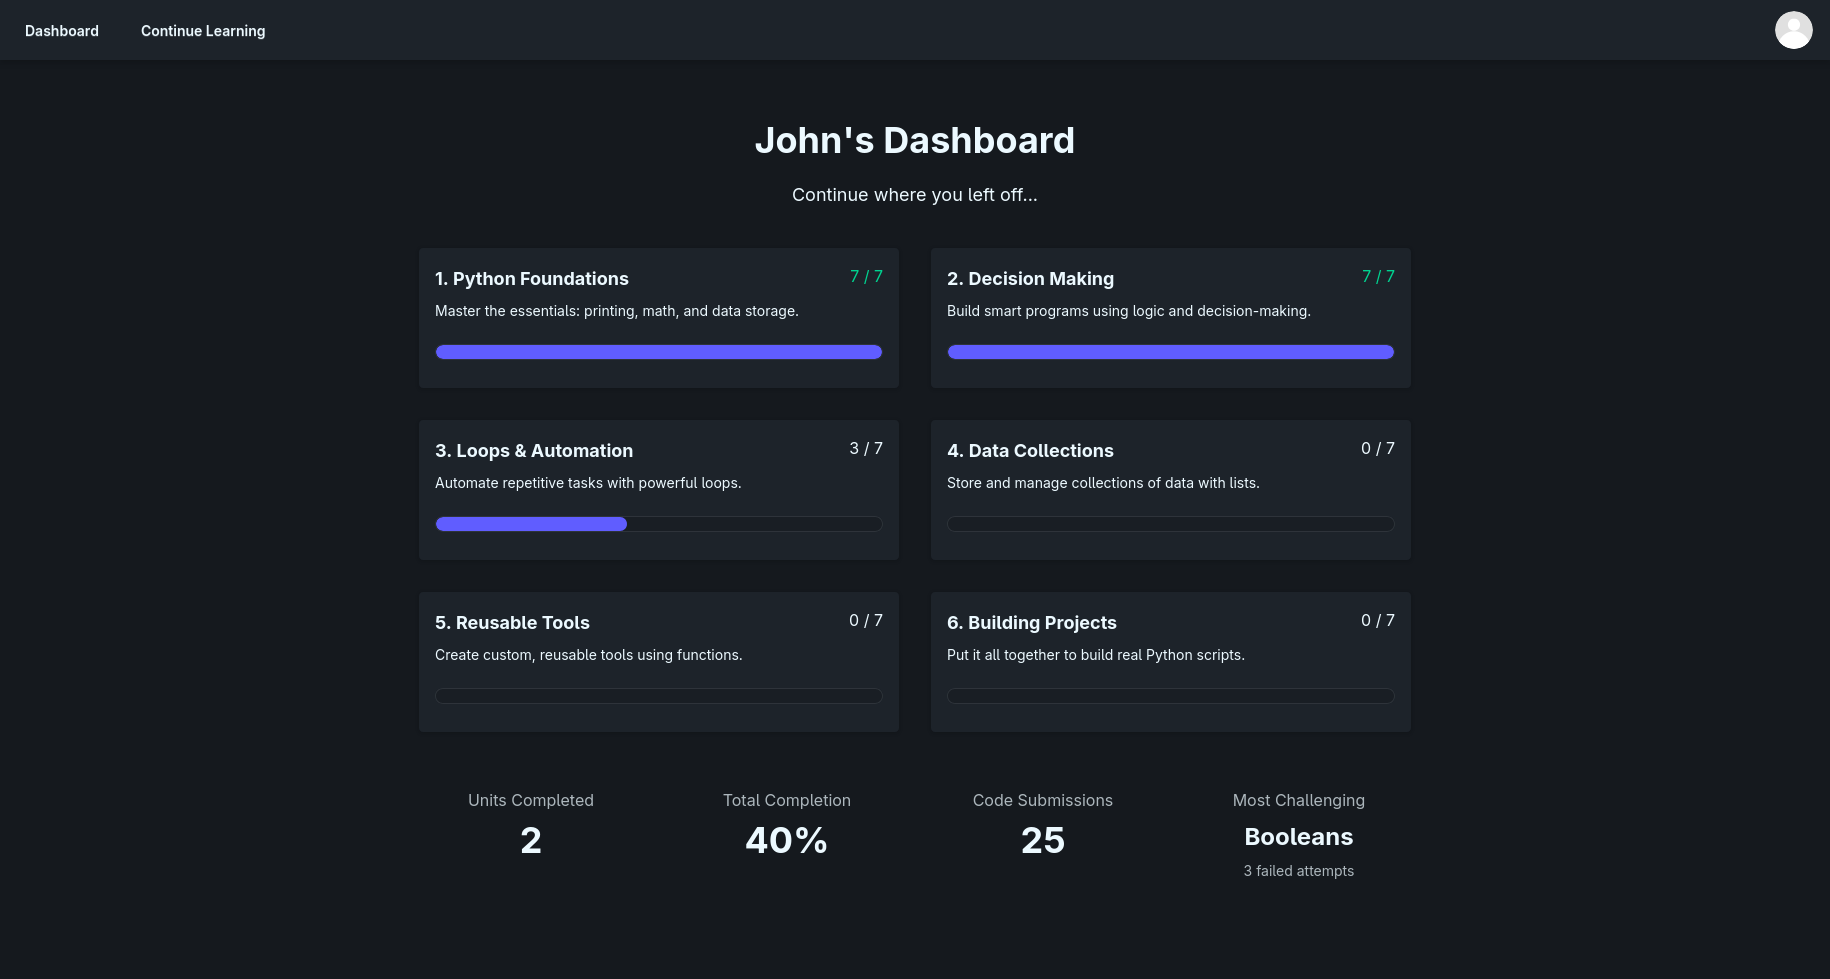
\includegraphics[width=0.9\textwidth]{screenshots/dashboard_stats.png} 
    \caption{The main application layout demonstrating consistent DaisyUI thematic application.}
    \label{fig:main_layout}
\end{figure}

\section{Semantic Layering and Visual Hierarchy}
In educational software, it is crucial to visually distinguish between theoretical instruction and interactive activities. The application employs "Semantic Layering" through DaisyUI's base color tokens. 

The primary reading area (theory) utilizes the primary background token (\texttt{bg-base-100}). Conversely, interactive elements—such as the Piston-powered terminal output and the \texttt{react-syntax-highlighter} code examples—are rendered atop a darker \texttt{bg-base-200} layer. This creates a "sunken" or "well" visual effect, instinctively signaling to the student that the enclosed content is an interactive or technical component requiring active attention. 

Furthermore, to maintain aesthetic integrity, prop-level style overrides were applied to third-party libraries (e.g., \texttt{react-syntax-highlighter}) to strip away their default internal borders and background colors. This forces the components to inherit the application's native DaisyUI theme, resulting in a seamless, bespoke UI rather than a disjointed collection of plugins.

\section{Typography System for Code Legibility}
Reading code is fundamentally different from reading prose. The typography system was specifically tuned to prioritize legibility and syntax recognition during the transcription phase of the self-assessment activities.

\subsection{Sizing and Spacing}
The \texttt{CodeEditor} and Markdown \texttt{code} blocks utilize an increased font size (\texttt{1.1rem}) and generous line-spacing ($1.6\times$). This specific ratio prevents visual crowding, making it significantly easier for absolute beginners to spot critical syntax details, such as the difference between parentheses \texttt{()} and brackets \texttt{[]}.

\subsection{UX Optimization for Novice Learners (Ligature Prevention)}
Modern programming fonts often employ "font ligatures" (Contextual Alternates), which combine contiguous characters into single aesthetic glyphs (e.g., rendering \texttt{<=} as a mathematical "less than or equal to" symbol). While popular among experienced developers, this abstraction is pedagogically harmful to absolute beginners who must map on-screen code directly to their physical keyboards.

To prevent pedagogical confusion during the introduction of logical and comparison operators in Unit 2, the application's global CSS explicitly disables these typographic features.

By forcing the browser to render composite operators exactly as they are typed, the application minimizes syntax errors and reduces beginner frustration, directly answering the rubric's call for a "carefully designed user interface" tailored to the target audience.

\begin{figure}[htbp]
    \centering
    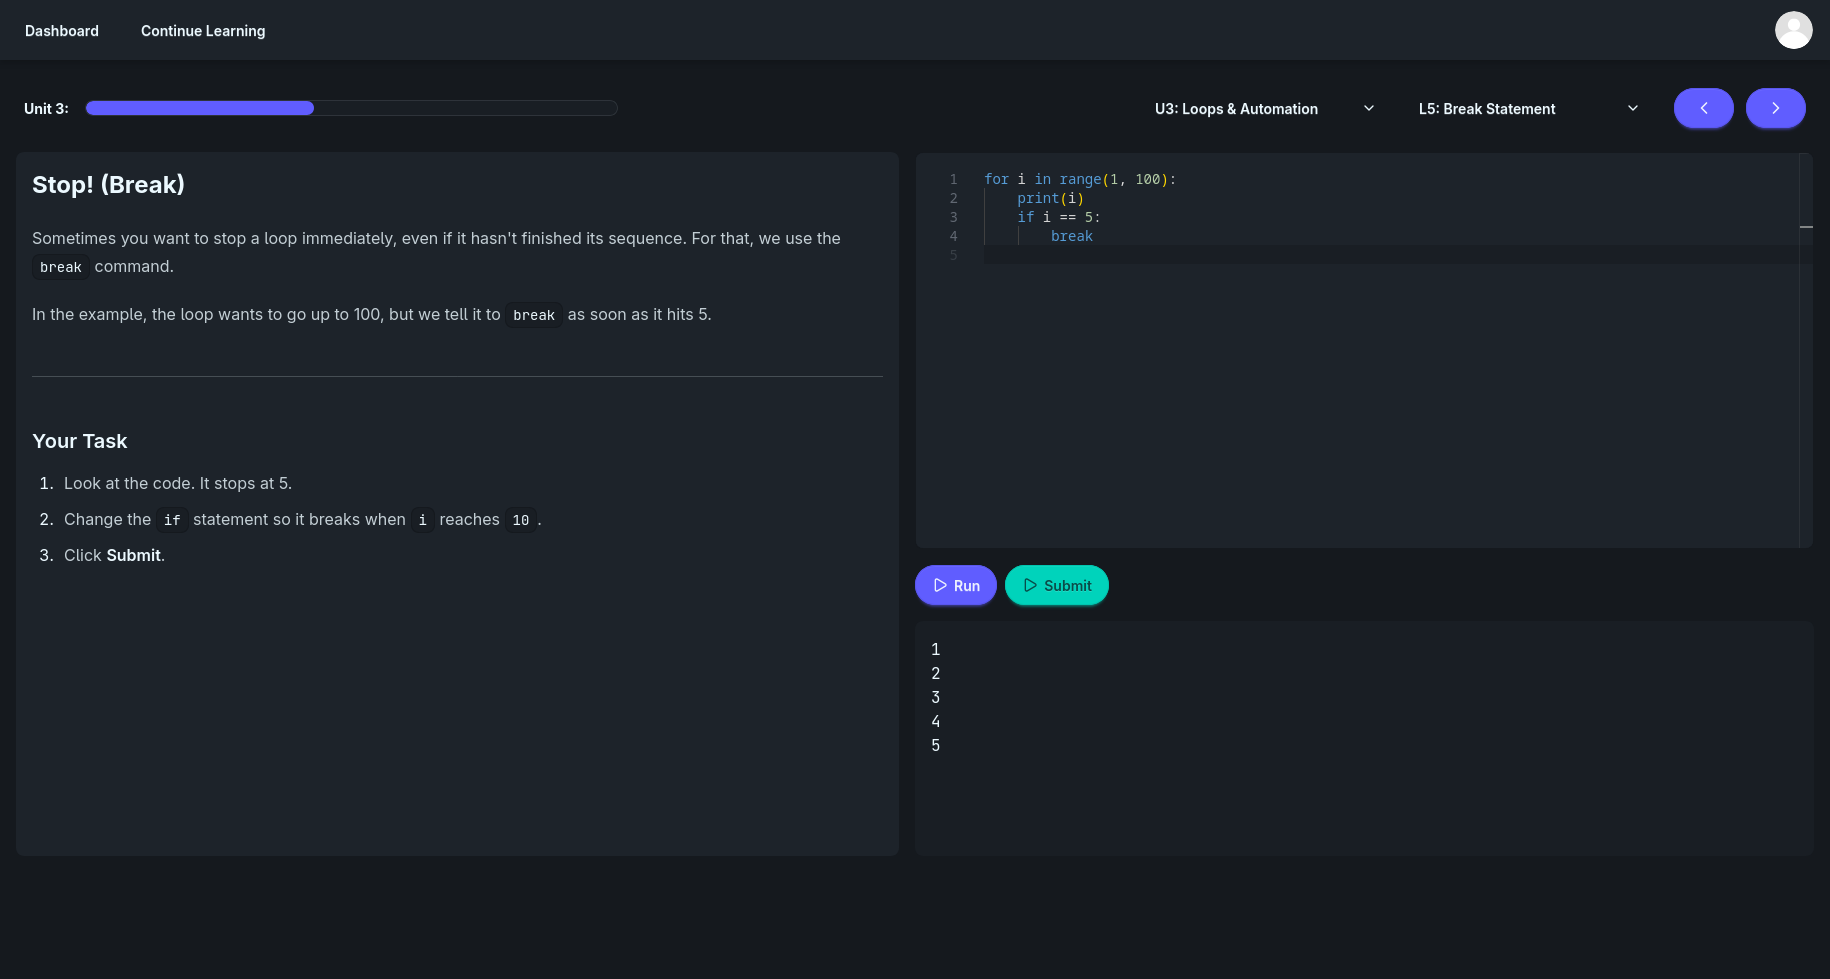
\includegraphics[width=0.9\textwidth]{screenshots/lesson_ui.png}
    \caption{Code view demonstrating increased line-height and disabled ligatures for clarity.}
    \label{fig:typography_view}
\end{figure}

\chapter{Self-Assessment}
Lorem Ipsum...


\end{document}
